\documentclass[10pt]{article}
\usepackage[pdftex]{graphicx, color}
\usepackage{listings}
\usepackage{amsmath}
\usepackage{amsfonts}
\usepackage{amssymb}
\usepackage{mathtools} 
\usepackage{tikz}
\usepackage{qtree}
\usepackage{hyperref}
\usepackage{multirow}
\usepackage{ulem}
\usepackage{seqsplit}
\usepackage{tikz-qtree}
\usepackage{float}

\usetikzlibrary{automata,positioning}

\headheight 8pt \headsep 20pt \footskip 30pt
\textheight 9in \textwidth 6.5in
\oddsidemargin 0in \evensidemargin 0in
\topmargin -.35in

\newcommand {\pts}[1]{({\bf #1 pts})}
\newcommand {\response}{{\color{blue}\textbf{RESPONSE:}\\}}

\lstset{basicstyle=\small\ttfamily,breaklines=true}

\begin{document}


\begin{center}
	\Large CS131 Compilers: Writing Assignment 1\\Due 11:59pm April 2, 2023
\end{center}



\begin{center}
	%% Change this:
	\LARGE Name - ID
\end{center}




\begin{center}
	%% Change this:
	I worked with Name1 Name2 ...
	\small \\Complteted on \today
\end{center}

\begin{center}
	\large \textbf{Code of Conduct}    \\
\end{center}

\small \textbf{This writing assignment should be your own individual work. Discussion on concept, methodology, and class materials are welcomed, but you should list all the people you have discussed with. Copying is strictly prohibited. Plagiarism, once confirmed, may result in assignment grades reduced to zero for all involved people. And this event will be reported. Also you should use \LaTeX \ to produce your response based on this template. Submission in other forms won't be graded.}\\


\begin{figure}[h]
\centering
	{\Tree [.. [.. [.a ][.* [.+ [.b ][.c ]] ] ][.\# ]]}
	\caption{Simple Tree drawn by Tikz-qtree package}
	\label{fig:tikz2}
\end{figure}

\begin{figure}[h]
	\centering
	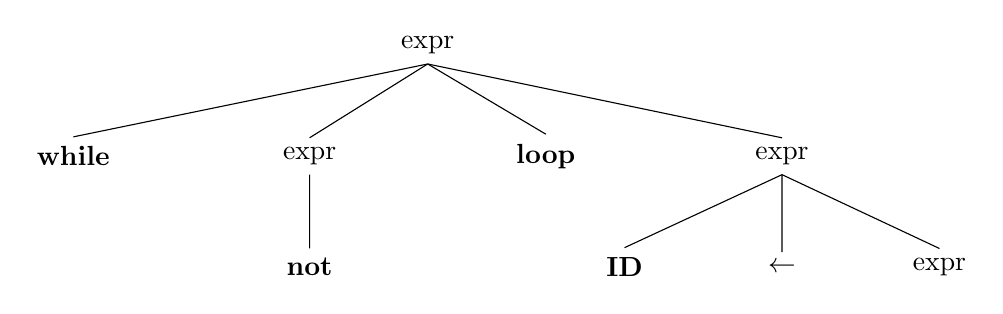
\begin{tikzpicture}    [
        level distance = 4em,
	    level 1/.style={sibling distance=3cm},
	    level 2/.style={sibling distance=2cm},
	    level 3/.style={sibling distance=1.5cm}
    	]
        \node(root){expr}
        	child{node{\textbf{while}}}
        	child{node{expr}
        		child{node{\textbf{not}}}
        	}
        	child{node{\textbf{loop}}}
        	child{node{expr}
        		child{node{\textbf{ID}}}
				child{node{$\leftarrow$}}
				child{node{expr}}
        	};

        \end{tikzpicture}
	\caption{Complex tree Drawn by Tikz package}
	\label{fig:tikz0}
\end{figure}

\begin{figure}[h]
	\centering
	\begin{center}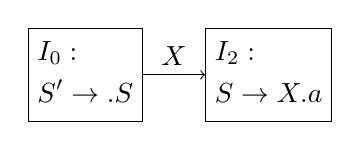
\begin{tikzpicture}[]
		\node[state,shape=rectangle] (I0) { 
		    $
			\begin{aligned}
				& I_0: \\
				& S' \rightarrow .S \\
			\end{aligned}
			$
		};
		\node[state, right of=I0, shape=rectangle,node distance=2.33cm] (I1){
		    $
			\begin{aligned}
				& I_2: \\
				& S\rightarrow X.a \\
			\end{aligned}
			$
		};		
		\path[->]
		(I0) 	edge 					node[above]{$X$} (I1);
	\end{tikzpicture}\end{center}
	\caption{Item automata drawn by Tikz package}
	\label{fig:automata}
\end{figure}

\begin{figure}[H]
    \centering
    \begin{tabular}{|c|ccccc||cccc|}
		\hline
		\multirow{2}{*}{STATE} & \multicolumn{5}{c||}{ACTION}                                                                                 & \multicolumn{4}{c|}{GOTO}                                                     \\ \cline{2-10} 
		& \multicolumn{1}{c|}{(}  & \multicolumn{1}{c|}{)}  & \multicolumn{1}{c|}{q}  & \multicolumn{1}{c|}{a}  & \$  & \multicolumn{1}{c|}{E} & \multicolumn{1}{c|}{T} & \multicolumn{1}{c|}{Q} & A  \\ \hline
		0                      & \multicolumn{1}{c|}{s2} & \multicolumn{1}{c|}{}   & \multicolumn{1}{c|}{}   & \multicolumn{1}{c|}{}   &     & \multicolumn{1}{c|}{1} & \multicolumn{1}{c|}{}  & \multicolumn{1}{c|}{}  &    \\ \hline
		1                      & \multicolumn{1}{c|}{}   & \multicolumn{1}{c|}{}   & \multicolumn{1}{c|}{}   & \multicolumn{1}{c|}{}   & acc & \multicolumn{1}{c|}{}  & \multicolumn{1}{c|}{}  & \multicolumn{1}{c|}{}  &    \\ \hline
		2                      & \multicolumn{1}{c|}{}   & \multicolumn{1}{c|}{}   & \multicolumn{1}{c|}{s6} & \multicolumn{1}{c|}{}   &     & \multicolumn{1}{c|}{}  & \multicolumn{1}{c|}{3} & \multicolumn{1}{c|}{4} &    \\ \hline
		3                      & \multicolumn{1}{c|}{}   & \multicolumn{1}{c|}{}   & \multicolumn{1}{c|}{}   & \multicolumn{1}{c|}{}   & r1  & \multicolumn{1}{c|}{}  & \multicolumn{1}{c|}{}  & \multicolumn{1}{c|}{}  &    \\ \hline
		4                      & \multicolumn{1}{c|}{}   & \multicolumn{1}{c|}{s5} & \multicolumn{1}{c|}{}   & \multicolumn{1}{c|}{}   &     & \multicolumn{1}{c|}{}  & \multicolumn{1}{c|}{}  & \multicolumn{1}{c|}{}  &    \\ \hline
		5                      & \multicolumn{1}{c|}{}   & \multicolumn{1}{c|}{}   & \multicolumn{1}{c|}{}   & \multicolumn{1}{c|}{}   & r2  & \multicolumn{1}{c|}{}  & \multicolumn{1}{c|}{}  & \multicolumn{1}{c|}{}  &    \\ \hline
		6                      & \multicolumn{1}{c|}{}   & \multicolumn{1}{c|}{}   & \multicolumn{1}{c|}{r5} & \multicolumn{1}{c|}{s9} &     & \multicolumn{1}{c|}{}  & \multicolumn{1}{c|}{}  & \multicolumn{1}{c|}{}  & 7  \\ \hline
		7                      & \multicolumn{1}{c|}{}   & \multicolumn{1}{c|}{}   & \multicolumn{1}{c|}{s8} & \multicolumn{1}{c|}{}   &     & \multicolumn{1}{c|}{}  & \multicolumn{1}{c|}{}  & \multicolumn{1}{c|}{}  &    \\ \hline
		8                      & \multicolumn{1}{c|}{}   & \multicolumn{1}{c|}{r3} & \multicolumn{1}{c|}{}   & \multicolumn{1}{c|}{}   &     & \multicolumn{1}{c|}{}  & \multicolumn{1}{c|}{}  & \multicolumn{1}{c|}{}  &    \\ \hline
		9                      & \multicolumn{1}{c|}{}   & \multicolumn{1}{c|}{}   & \multicolumn{1}{c|}{r5} & \multicolumn{1}{c|}{s9} &     & \multicolumn{1}{c|}{}  & \multicolumn{1}{c|}{}  & \multicolumn{1}{c|}{}  & 10 \\ \hline
		10                     & \multicolumn{1}{c|}{}   & \multicolumn{1}{c|}{}   & \multicolumn{1}{c|}{r4} & \multicolumn{1}{c|}{}   &     & \multicolumn{1}{c|}{}  & \multicolumn{1}{c|}{}  & \multicolumn{1}{c|}{}  &    \\ \hline
\end{tabular}
    \caption{A parser table (generated by LatexTable Generator)}
    \label{fig:table}
\end{figure}

\begin{figure}[H]
    \centering
    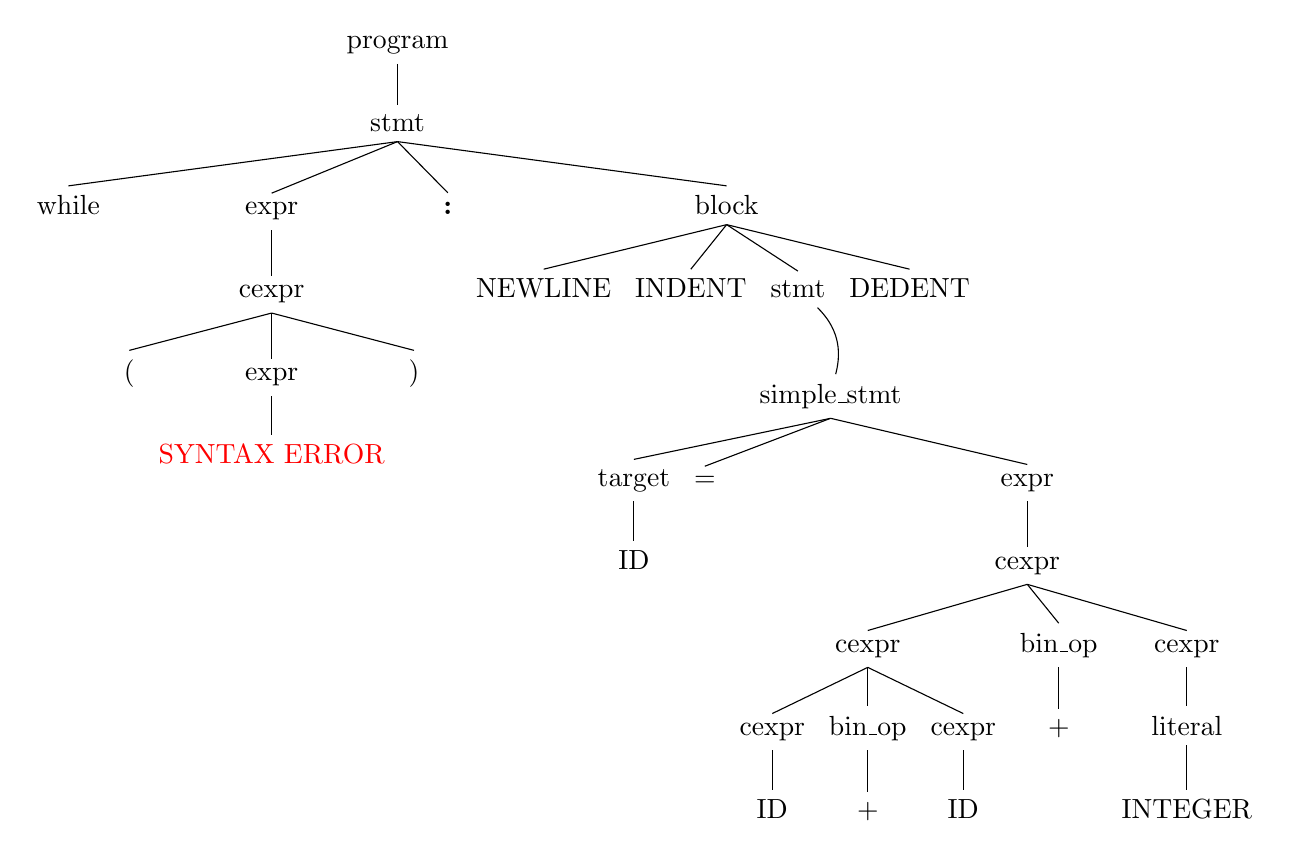
\begin{tikzpicture}
    
			\Tree [.program [.stmt [.while ][.expr [.cexpr 
				[.( ] [.expr {\color{red}SYNTAX ERROR} ] %[.cexpr [.cexpr ID ][.bin\_op \textbf{==} ][.cexpr [.literal INTEGER ]]][.bin\_op $<$ ][.cexpr [.literal INTEGER ]]]
				[.) ]
			]][.\textbf{:} ][.block NEWLINE INDENT [.\node(site){stmt}; ] DEDENT ]]]
			\begin{scope}[shift={(5.5cm,-4.5cm)}]
			\Tree [.\node(rt){simple\_stmt}; [.target ID ]$=$ [.expr [.cexpr [.cexpr [.cexpr ID ][.bin\_op $+$ ][.cexpr ID ]][.bin\_op $+$ ][.cexpr [.literal INTEGER ]]]]]
			\end{scope}
			\draw (site) edge[bend left] node{}(rt);
\end{tikzpicture}
    \caption{A very large tree drawn by Tikz package}
    \label{fig:my_label}
\end{figure}

\begin{figure}[H]
    \centering
    $$
    \begin{aligned} S_{\epsilon} & \to \epsilon \\ 
        S_{c \in \Sigma} & \to c_1|c_2|\dots|c_{|\Sigma|}\\ 
        S_{A B} & \to S_AS_B \\ 
        S_{A+B} & \to S_A|S_B\\
         S_{A^{*}} & \to S_AS_{A^*}|\epsilon
         \end{aligned}
         $$
    \caption{a context Free grammar that can represent a regular expression}
    \label{fig:cfg}
\end{figure}

\newpage
\begin{enumerate}
	\item \pts{$2 +2 +2+2+2 + 4 + 4 =18$} For each of the following question, write a \textbf{short and clear} answer.\\
	    (Hint: All answers can be found according to slides and textbook.)
	      \begin{enumerate}
	        \item Did you start your PAs and find one teammate? Who is he/she/they?\\\response
	        \item Context Free Grammar(CFG) can be described by $(\mathcal{T},\mathcal{NT},\mathcal{S},\mathcal{P})$. What are they? \\\response
	      	\item What do ``\textbf{Leftmost}" and ``\textbf{Rightmost}" mean in \textbf{derivation}?\\\response
	      	\item What is the \textbf{Ambiguity} of a grammar? Then name two methodology to solve \textbf{Ambiguity}.\\\response
	      	\item What is \textbf{Predictive Parser} and \textbf{Recursive Descent Parser}?   \\\response
	      	\item $\forall x \in \{L,R,S,A,k\}$, what does $x$ mean in the following expressions?\\
	      	\begin{enumerate}
	      	    \item LL(k) \\\response 
	      	    \item LR(k) \\\response
	      	    \item SLR   \\\response
	      	    \item LALR  \\\response
	      	\end{enumerate}
	      	\item If you are given a \textbf{conflict-free LR(1)} automaton, how can you get a \textbf{LALR(1)} parse table from it? \\(Give a short and clear answer) \\\response
	      \end{enumerate}
	\item \pts{$2+2+2+4=10$} Write a relevant CFG or draw a parser(ie. pushdown automata, but not recommended) that correctly represents the context free language described in each question. Your response should be sound and complete.
	      \begin{enumerate}
	      	\item $L_1=\{ (^k)^k|k=0,1,2,3,\dots\}$\\
	      	      \response 
	      	\item $L_2=\big\{\text{All non-empty Palindrome strings over }\Sigma=\{0,1\}\big\}$\\
	      	      \response
	      	\item $L_3=L_1 + L_2=L_1\cup L_2$\\
	      	      \response
	        \item $L=\{\textbf{a}^n \textbf{b}^n \textbf{c}^m \textbf{d} | m,n \ge 0\} \cup \{\textbf{a}^n \textbf{b}^m \textbf{c}^m \textbf{e} | m,n \ge  0\}$\\	        (Note: this language is unambiguous but has not a unambiguous grammar.)
\\\response
	      \end{enumerate}
	      \newpage
	\item \pts{$3+3+3+6+6+9=30$} Consider this grammar $G_1$ (simplified from ChocoPy): 
	    $$
	    \begin{aligned}
	        expr &\to binary|\textbf{id}|expr \textbf{ if } expr \textbf{ else } expr\\
	        binary &\to expr\ op \ expr\\
	        op &\to \textbf{and} | \textbf{or}\\
	    \end{aligned}
	    $$
	    Where $expr$ is the start symbol.
	      \begin{enumerate}
	      	\item How many different \textbf{leftmost derivation} parsing trees are there of
	      	$$
	      	\textbf{id and id or id if id else id}
	      	$$\response
	      	\item Do Left-recursion elimination on the grammar $G_1$, show me the converted grammar $G_2$.\\\response
	      	\item Do Left-factoring on the grammar $G_2$, show me the converted grammar $G_3$.\\\response
	      	\item Consider \textbf{LL(1)}. Compute the \textbf{FIRST} and the \textbf{FOLLOW} function of the grammar $G_3$. \\\response
	      	\item Construct the \textbf{LL(1)} parse table of $G_3$. Then tell whether $G_3$ is \textbf{LL(1)} grammar.\\\response
	      	\item Suppose the precedence is $\textbf{and} > \textbf{or} > \textbf{if-else}$. Also, suppose $\textbf{and},\textbf{or}$ are left-associative, and \textbf{if-else} is right-associative. Design a new context free grammar $G_1'$ that remove all ambiguity and $L(G_1) = L(G'_1)$. Left-associative means \\ ($L(G)$ means the set of all strings that the grammar $G$ can represent. )\\ 
	      	The correct grammar would parse the following input:
	      	$$
	      	\textbf{id or id and id or id if id else id and id if id else id}
	      	$$
	      	to some derivation trees like the below. \textbf{This tree is not the final parse tree.} It only illustrates the tree structure of operators by the structures of terminals(ie. leaves), which indicates the order of calculating(father computed after decedents, and this is how operator precedence is solved in real world). \\
	      	\begin{center}
	      	    \Tree[.E [.E [.E [.E \textbf{id} ] \textbf{or} [.E [.E \textbf{id} ] \textbf{and} [.E \textbf{id} ] ] ] \textbf{or} [.E \textbf{id} ] ] \textbf{if} [.E \textbf{id} ] \textbf{else} [.E [.E \textbf{id} ] \textbf{if} [.E \textbf{id} ] \textbf{else} [.E \textbf{id} ] ] ]
	      	\end{center}
	      	\response
	      \end{enumerate}
	      \newpage
	      % In fact, a context free language has any unambiguous context free grammar if and only if an LR(1) parser of it without conflict can be constructed. The Contrary proposition  also holds.
	      \item \pts{$3+4+4+6+4=21$} Consider the following grammar $G_4$, simplified from the ChocoPy.
	      $$
	      \begin{aligned}
	           stmt &\to\textbf{if }expr\textbf{ : }block\textbf{ else : }block\\
	           stmt &\to\textbf{if }expr\textbf{ : }block\\
	          block &\to\textbf{NEWLINE INDENT } \textbf{ID} \textbf{ DEDENT }\\
	          expr &\to \textbf{ID} 
	      \end{aligned}
	      $$
	      where $stmt$ is the start symbol. You can use abbreviation \textbf{NL}, \textbf{IND}, \textbf{DED} for long terminals.
	      \begin{enumerate}
	          \item Suppose we use LR(0) technique, identify \textbf{one shift-reduce conflicts} by constructing the items automata. You don't need to draw the whole automata. \textbf{Instead, draw the sets of items(ie. the states in the automaton) where the conflicts occur.} \\\response
	          \item To construct at SLR(1) parser, Compute FIRST function and FOLLOW function of each Non-terminals. \\\response
	          \item Construct the SLR items automaton. The process is not required. \\\response
	          \item Based on the SLR items automaton, construct the parsing table. The process is not required. Please refer to the format in the lectures or in the preface \ref{fig:table}. \\\response
	          \item Based on your parse table, parse this input sequence to a parse tree. 
	          $$
	          \textbf{if ID : NEWLINE INDENT ID DEDENT}
	          $$\\\response
	      \end{enumerate} 
	      \newpage
	      \item \pts{$15+4+4 = 23$}Consider the CFG below
	      $$
	      \begin{aligned}
S &\to X\ X\\
X &\to \textbf{a}\ X\\ 
X &\to \textbf{b}     \\
	      \end{aligned}    
	      $$
	      \begin{enumerate}
	   \item Construct the LALR(1) parse table. \textbf{The process is not required. But showing your process may save your score if your answer is accidentally wrong.}
	   \begin{enumerate}
	       \item Build LR(1) items automata (optional)
	       \item Build the LALR(1) parse table. (required)
	   \end{enumerate}\response
	      \item Use your parse table, parse the following input. Your response should include the all configurations from the initial state to the ending state.
	      $$
	      \textbf{a a a b b}
	      $$\response
	      \item Build the parse tree of the input above. \\\response
	      \end{enumerate}
\end{enumerate}
\vfill
\hrule
\center{\large\textbf{End of This Assignment}}

\end{document}